\section{Задание}

Смоделировать систему, состоящую из генератора, очереди и обслуживающего аппарата.
Закон генерации заявок выбирается равномерный.
Закон в ОА берется из лабораторной работы \textnumero1.
Определить оптимальную длину очереди, т.е. ту длину, при которой ни одно сообщение не исчезает.
Должна быть возможность возвращения заявки в
очередь после ее обработки с заданной вероятностью.


\section{Теоритическая часть}

\subsection{$\Delta t$ принцип}

Принцип $\Delta t$ заключается в последовательном анализе состояний всех блоков в момент $t + \Delta t$ по заданному состоянию блоков в момент $t$. При этом новое состояние блоков определяется в соответствии с их алгоритмическим описанием с учетом действующих случайных факторов, задаваемых распределениями вероятности. В результате такого анализа принимается решение о том, какие общесистемные события должны имитироваться программной моделью на данный момент времени.

Достоинство: равномерная протяжка времени.

Недостаток: значительные затраты машинного времени на реализацию моделирования системы. А при недостаточно малом $\Delta t$ появляется опасность пропуска отдельных событий в системе, что исключает возможность получения адекватных результатов при моделировании.

\subsection{Событийный принцип}

Характерное свойство моделируемых систем -- состояние отдельных устройств изменяется в дискретные моменты времени, которые совпадают с моментами поступления сообщений в систему, моментами окончания решения задач, моментами возникающих аварийных сигналов и т.д. Поэтому, моделирование и продвижение текущего времени в системе удобно проводить использую событийный принцип, при котором состояние всех блоков системы анализируется лишь в момент наступления какого-либо события.

Момент наступления следующего события определяется минимальным значением из списка будущих событий, представляющих собой совокупность моментов ближайшего изменения состояний каждого из блоков системы.


Достоинство: не пропустим ни одного события

Недостаток: при большом количестве событий (сложная система) список необходимо просматривать
постоянно (можно держать сортированным).

\section{Результаты}

\begin{figure}[h!]
\centering
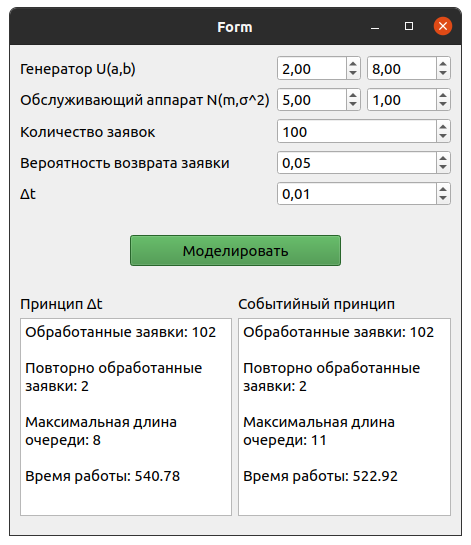
\includegraphics[width=0.52\textwidth]{4/ex_1}
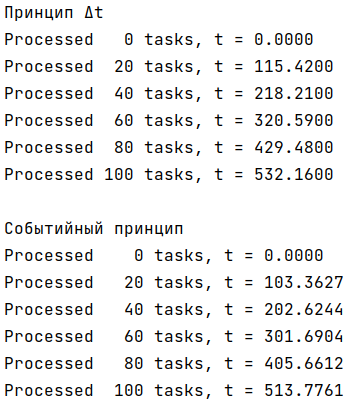
\includegraphics[width=0.38\textwidth]{4/ex_1_log}
\caption{Среднее время между поступлением задачи = среднее время обработки задачи, вероятность возврата небольшой, размер очереди немного увеличивается}
\end{figure}

\begin{figure}[h!]
\centering
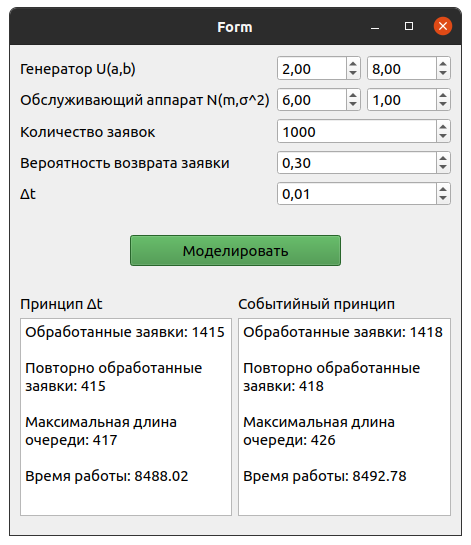
\includegraphics[width=0.52\textwidth]{4/ex_2}
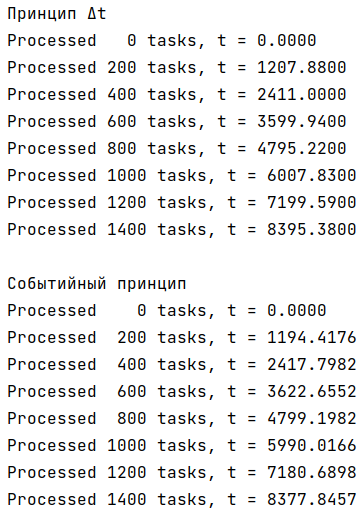
\includegraphics[width=0.38\textwidth]{4/ex_2_log}
\caption{Среднее время между поступлением задачи < среднее время обработки задачи, вероятность возврата = 0.3, размер очереди значительно увеличивается.}
\end{figure}


\pagebreak
\section{Листинг кода}

\lstinputlisting[language=Python, caption=Программная реализация обслуживающего аппарата]{../4/system/model.py}
